\section{Consensus and Application Data}

To pinpoint exactly our contributions to optimizations in
consensus data, in this section we review the difference between
\emph{application data} and \emph{consensus data} which was
discussed in Chapter~\ref{chapter:background}.

Blockchain systems maintain certain \emph{application state}.
This state can be used to, for example, determine who owns how much
money. There are two primary ways of representing ownership
in today's blockchains: A \emph{UTXO}-based system, in which the application
state is comprised of the \emph{unspent transaction outputs} that
remain available for spending; and an \emph{accounts}-based system,
in which the application state is comprised of \emph{accounts and
their balances}. The first one is used primarily by Bitcoin, while
the second one is used by Ethereum.

The application state evolves over time when \emph{transactions} are applied
to it. A transaction is a state evolution operator applied on the application
state. Given a previous application state and a transaction, a new application
state can be computed. Each block in the chain contains multiple transactions
in a particular order. As such, a block is itself a state evolution operator
which applies multiple transactions in order. By applying a block to a previous
application state, a new application state can be computed.

There are two schools of thought regarding what should be stored in a
block. In the first school of thought, only transactions (deltas) are stored. The
application state at the end of the blockchain can be computed by
starting at the \emph{genesis} application state (an \emph{empty} application
state) and \emph{traversing} the blockchain, applying the state evolution
described by each block, in order, and arriving at the final application state.
This is what Bitcoin does. The other school of thought stores both transactions
and the state \emph{after} these transactions have been applied, a so-called
\emph{snapshot}. In such
systems, if one holds the longest chain, the application state at the end of
the chain does not need to be computed by applying any deltas.
Instead, a block near the end of the chain can simply be inspected and the application state
within it extracted.

It is possible to apply either school of thought to either application
state model. Bitcoin only keeps only deltas for a UTXO-based application state.
However, nothing prevents Bitcoin from committing to the newly computed UTXO
in every block~\cite{rollerchain,bitcoin-prune,utreexo}, and in fact some Bitcoin
forks have already done so. On the other hand, Ethereum keeps both deltas and
snapshots in blocks. While the snapshots are not necessary, they are helpful.
For the rest of this chapter, \emph{we assume a proof-of-work blockchain in which
each block commits to an application state snapshot}. The exact application state
format (UTXO, accounts, or something else) is irrelevant for our purposes.

In both schools of thought, it is imperative that the validity of the application
data (deltas or snapshots) is verified before a block can be accepted as valid.
For example, in a snapshotted system, miners must check that the snapshot committed
to a block was obtained by applying the transactions to the previous snapshot.

Let us now discuss how a bootstrapping node can synchronize with the rest of the
network. A bootstrapping node is a node holding only the \emph{genesis} block and
booting for the first time. A wallet node is interested in the \emph{current} application
state that concerns it. For example, it is interested to learn which UTXOs it owns,
or how much money is in its own accounts. The \emph{custodial history} of how these
assets came to belong to it is irrelevant~\cite{utreexo}, beyond archival purposes, as long as it
can be sure that the
assets it holds correspond to the correct application state based on the history
that took place. Inspecting or having access to this history itself is not important
for consensus purposes.
As such, this node can synchronize with the rest of the network using the \emph{SPV}
method~\cite{bitcoin}: It downloads only the block \emph{headers} to determine which chain
is the longest one. It then inspects a block near the end of the chain and
extracts the balance from the Merkle tree leaf for its own accounts, or for its UTXOs.
This is sufficient to know the assets that it owns.
In case some nodes are interested in the history of the blockchain, this history
can be maintained by special archival nodes or block explorers, but are not
necessary for the maintenance of the security of the network.

A miner bootstrapping their node can function in a similar manner: Download
only the block headers to determine the longest chain, then inspect a block
near the end of the chain to obtain the application state snapshot. Contrary
to a wallet node, the miner must obtain the whole application state so that it
can validate new pending transactions as they arrive. As such, the miner downloads
the \emph{headers} for the whole chain, and the \emph{full} blocks only for blocks near the
end of the chain.

To be more precise, after the longest chain has been
determined by comparing block header chain lengths, the $k^\text{th}$ block from the
end is inspected, its application state snapshot is extracted, and the deltas
in next $k$ blocks are applied. This is necessary because an adversary can place incorrect
snapshots in the most recent $k$ blocks of a blockchain (folklore wisdom
suggests $k = 6$ for Bitcoin). While that blockchain
will look valid and long to someone verifying only headers, it will have snapshots
corresponding to an incorrect application of deltas. However, the adversary
cannot modify blocks prior to that, due to Common Prefix.

Note here that the miner does not need to verify the veracity of all historical
transactions: If we assume that the majority of the computational power was
honest for the duration of history, this ensures that, at all times during the
execution, the longest chain represented the correct history of the world (with
the exception of up to $k$ blocks towards the end). Under the honest majority
assumption, this scheme is as secure as full mining (but see the Discussion section
at the end of this chapter for a more nuanced take on this argument under temporary dishonest majority).
This is contrary to schemes such as SPV mining in which no snapshots are available.

Application data can grow or shrink. UTXOs can be created or deleted, accounts and
smart contracts can be created, updated and destroyed. State variables within smart
contracts can also be constructed or destructed. \emph{How} the application data grows is
ap\-pli\-ca\-tion-de\-pen\-dent. Typically, the application data will increase as the execution
continues. There are several attempts to optimize the size of these
data~\cite{edrax,lightning,composable-lightning,cerberus,brick,starks,truebit}.
We remind the reader that, in this thesis, we do not focus on these.

Instead, we focus on the size of the \emph{consensus data}, that of block headers
$H(ctr \allowbreak \concat \allowbreak x \allowbreak \concat \allowbreak s)$.
Contrary to the application data, these data increase
at a constant linear rate, as block headers are added to the chain. No matter if
channels or rollups are used, block headers must keep getting added to the chain.
A system designed to survive for the centuries to come
must provision for the scalability of this ever-growing part.
Even the solutions above that only download block headers do not tackle that problem.
As we will
see, it is possible to reduce the consensus data and neither store nor communicate
all block headers.

A visualization of the comparison between application and consensus data is shown in
Figure~\ref{fig.data}. The consensus data (horizontal) grows at an expected
constant rate in time. The application data (vertical) may grow (or shrink)
depending on the application, and optimizations or pruning methods can be applied
on top of them.

\begin{figure}[h]
\begin{center}
  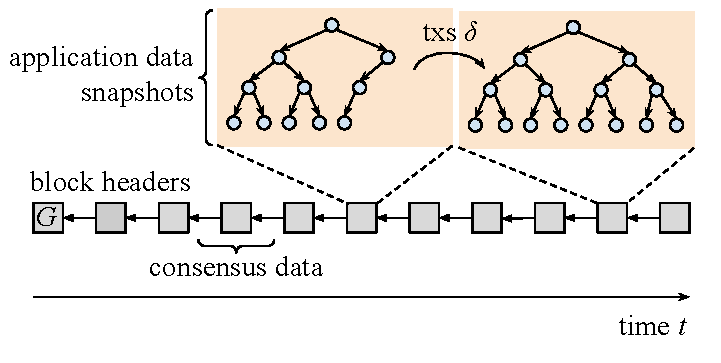
\includegraphics[width=0.8\columnwidth]{chapters/superlight/figures/data.pdf}
  \caption{A comparison of consensus data (growing horizontally with time) and
           application data (growing or shrinking vertically depending on the
           application).}
  \label{fig.data}
  \end{center}
\end{figure}

A comparison of our pruned mining construction against other constructions
(including the construction of Chapter~\ref{chapter:work})
is illustrated in Table~\ref{tab.comparison}.
In all of these protocols, we have a node (the \emph{prover}) that maintains all the necessary
state to help a newly booting node (the \emph{verifier} or \emph{client}) synchronize with the
rest of the network.  We compare the storage requirements for the prover, as well as the
communication complexity during bootstrapping. We are also interested
in whether, after synchronizing with the rest of the network, the verifier can function
as a fully-fledged miner on its own.

In this table, $n$ denotes the number of blocks in the chain, $\delta$ is the size of the
transactions in a single block (which may vary with time), $a$ is the size of the snapshot
or application state (which may also very with time), $c$ is the size of a block header, and
$k$ is the common prefix parameter, the number of blocks required for stability
(c.f.,~\cite{wallet-taxonomy}).
\emph{BTC Full} indicates the full bitcoin miner that synchronizes by downloading all
block headers and transactions $n(c + \delta)$.
\emph{BTC SPV} is a wallet-only client that downloads
only block headers and a single transaction, but requires the prover (the node that
serves it this data) to store the full history, as there are no snapshots available.
\emph{Ethereum} is a blockchain which uses block headers to synchronize, but makes use of
snapshots. Here, the prover can prune block contents, but not block headers (the $nc$ term
remains). For the last $k$ blocks, the transaction data of total size $k\delta$ are also needed to
verify the veracity of the tip of the chain; for the $k^\text{th}$ block from the end, only a
snapshot of size $a$ is needed.
The client can start mining on top of these snapshots (after the $k\delta$ transaction
data have been applied to the snapshot of size $a$).
Note that $a \leq n\delta$ and $k \leq n$, and so (asymptotically) $n(c + \delta) \geq nc + k\delta + a$.
\emph{Superblock} and \emph{FlyClient}
Charity NIPoPoWs (of Chapter~\ref{chapter:work}) allow a full node to function as a prover,
only sending consensus data
polylogarithmic in $n$, provided snapshots are available, but the receiving verifie
cannot function as a miner or a prover for others. In this chapter, we present a protocol
in which the verifier and prover both run on the same node. The prover is only required to store
polylogarithmic consensus data, and communication complexity is also polylogarithmic.
This is indicated by the term $poly\log(n)c$. The term $ka$, the application data,
remains unaffected.

\begin{table}[]
  \bgroup
  \def\arraystretch{1.1}
    \begin{tabular}{|r|r|r|r|}
    \hline
    \textbf{Proposal}            & \multicolumn{1}{l|}{\textbf{Storage}} & \multicolumn{1}{l|}{\textbf{Communication}} & \multicolumn{1}{l|}{\textbf{Can mine?}} \\ \hline
    \textbf{BTC Full}            & $n(c + \delta)$                       & $n(c + \delta)$                             & yes                                     \\
    \textbf{BTC SPV}             & $nc$                                  & $nc$                                        & no                                      \\
    \textbf{Ethereum}            & $nc + k\delta + a$                    & $nc + k\delta + a$                          & yes                                     \\
    \textbf{Chapter~\ref{chapter:work} NIPoPoWs} & $nc + k\delta + a$                    & $poly\log(n)c + k\delta + a$                & no                                      \\
    \textbf{FlyClient NIPoPoWs}  & $nc + k\delta + a$                    & $poly\log(n)c + k\delta + a$                & no                                      \\
    \textit{This chapter}           & $poly\log(n)c + k\delta + a$          & $poly\log(n)c + k\delta + a$                & yes                                     \\ \hline
    \end{tabular}
    \caption{A comparison of our results and other constructions. $n$: the number of blocks in the chain; $\delta$: size of transactions in a block; $c$: block header size; $a$: size of snapshot; $k$: common prefix parameter}
    \label{tab.comparison}
  \egroup
\end{table}
